\documentclass{beamer}
\usetheme{Rochester}
\usecolortheme{default}
%\setbeamercolor{structure}{fg=black}
\beamertemplatenavigationsymbolsempty

\usepackage[ngerman]{babel}
\usepackage{graphics}

\title{Hidden Markov Model als POS-Tagger für kleine, bedrohte Sprachen (Urum)}
\author{Aleksandr Schamberger}
\institute{Humboldt-Universität zu Berlin\\Institut für Slawistik und Hungarologie\\Einführung in die Computerlinguistik (mit Anwendung auf slawische Sprachen)\\WS 2023/24}
\date{\today}

\AtBeginSection[]{%
	\begin{frame}
		\frametitle{Gliederung}
		\tableofcontents[currentsection]
	\end{frame}
}

\begin{document}

\frame{\titlepage}

\begin{frame}[t]{Gliederung}
\tableofcontents
\end{frame}



\section{Was sind DoReCo und Urum?}

\subsection{DoReCo}

\begin{frame}{DoReCo: Language Documentation Reference Corpus}

\includegraphics[scale=0.5]{"./pics/doreco_logo.png"}
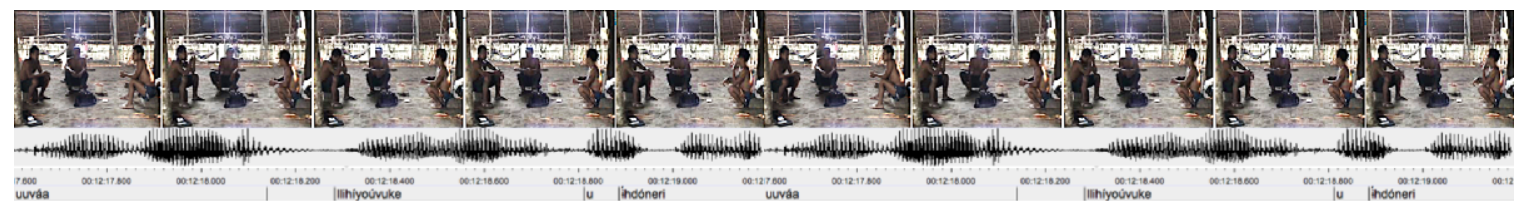
\includegraphics[scale=0.35]{"./pics/doreco_sublabel.png"}
\begin{itemize}
	\item Webseite des Projekts: \href{https://doreco.info/}{https://doreco.info/}
	\item Webseite des Repositoriums: \href{https://doreco.huma-num.fr/}{https://doreco.huma-num.fr/}
\end{itemize}
\end{frame}

\begin{frame}[t]{DoReCo: Language Documentation Reference Corpus}
	\begin{itemize}
		\item<1->DoReCo: Language \textbf{D}ocumentation \textbf{R}eference \textbf{C}orpus
		\item<2->weltweit 51 kleine, bedrohte Sprachen; ursprünglich gesammelt in der Feldforschung
		\item<3->Gesprochene Daten (mit Audioaufnahmen) meist erzählerischer (narrativer) Texte
		\item<4->Transkriptionen sind auf der Phon-Ebene \textbf{zeitaligniert}.
		\item<5->38 der 51 Sprachen verfügen über morphologische, zeitalignierte Annotationen
		\item<6->Korpusdaten (Transkriptionen/Annotationen) als eaf- (ELAN), TextGrid- und csv-Dateien
	\end{itemize}
\end{frame}

\begin{frame}{DoReCo: Beispiel in ELAN}
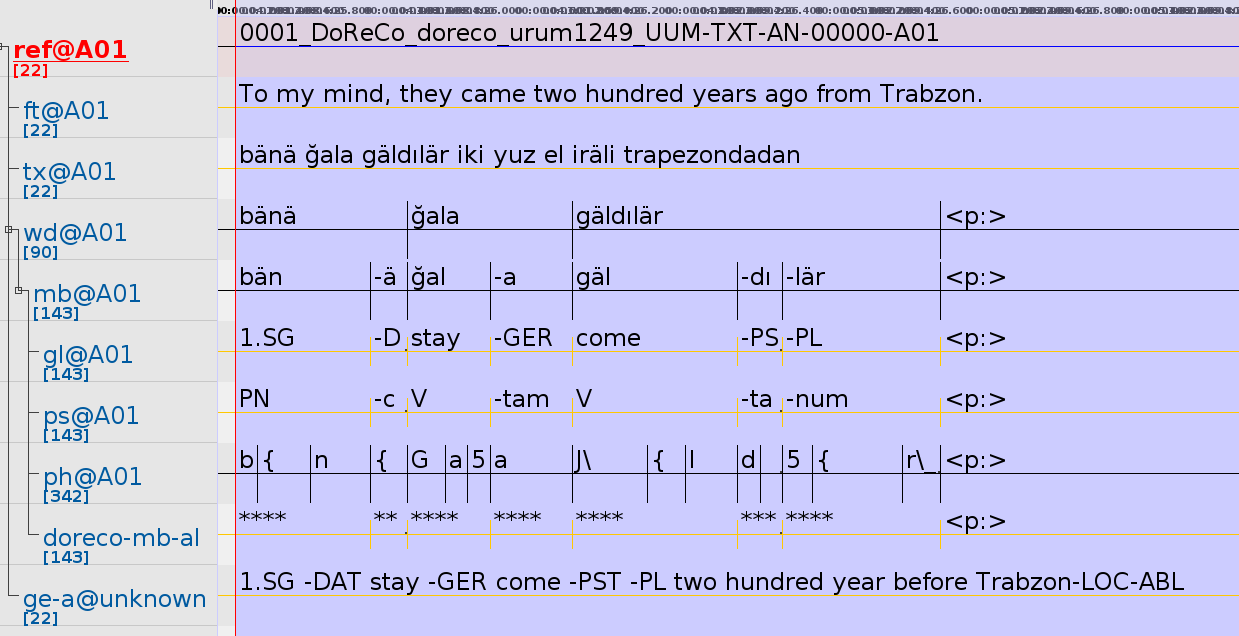
\includegraphics[scale=0.45]{./pics/urum_doreco_elan_example.png}
\end{frame}

\subsection{Urum}

\begin{frame}{Urum: DoReCo Karte}
	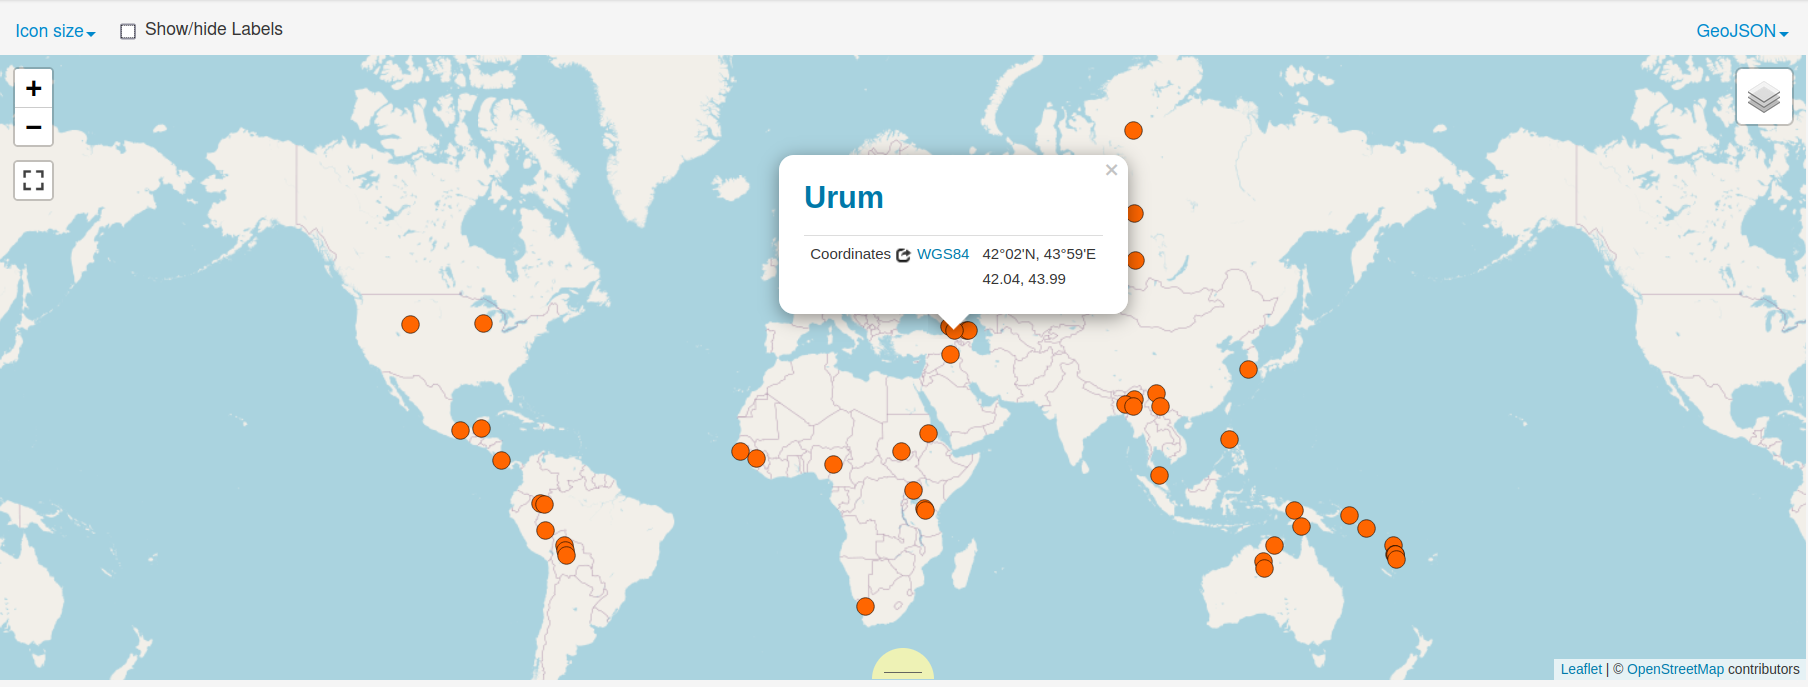
\includegraphics[scale=0.3]{./pics/urum_map_doreco.png}
\end{frame}

\begin{frame}{Urum: Karte: Genauer}
	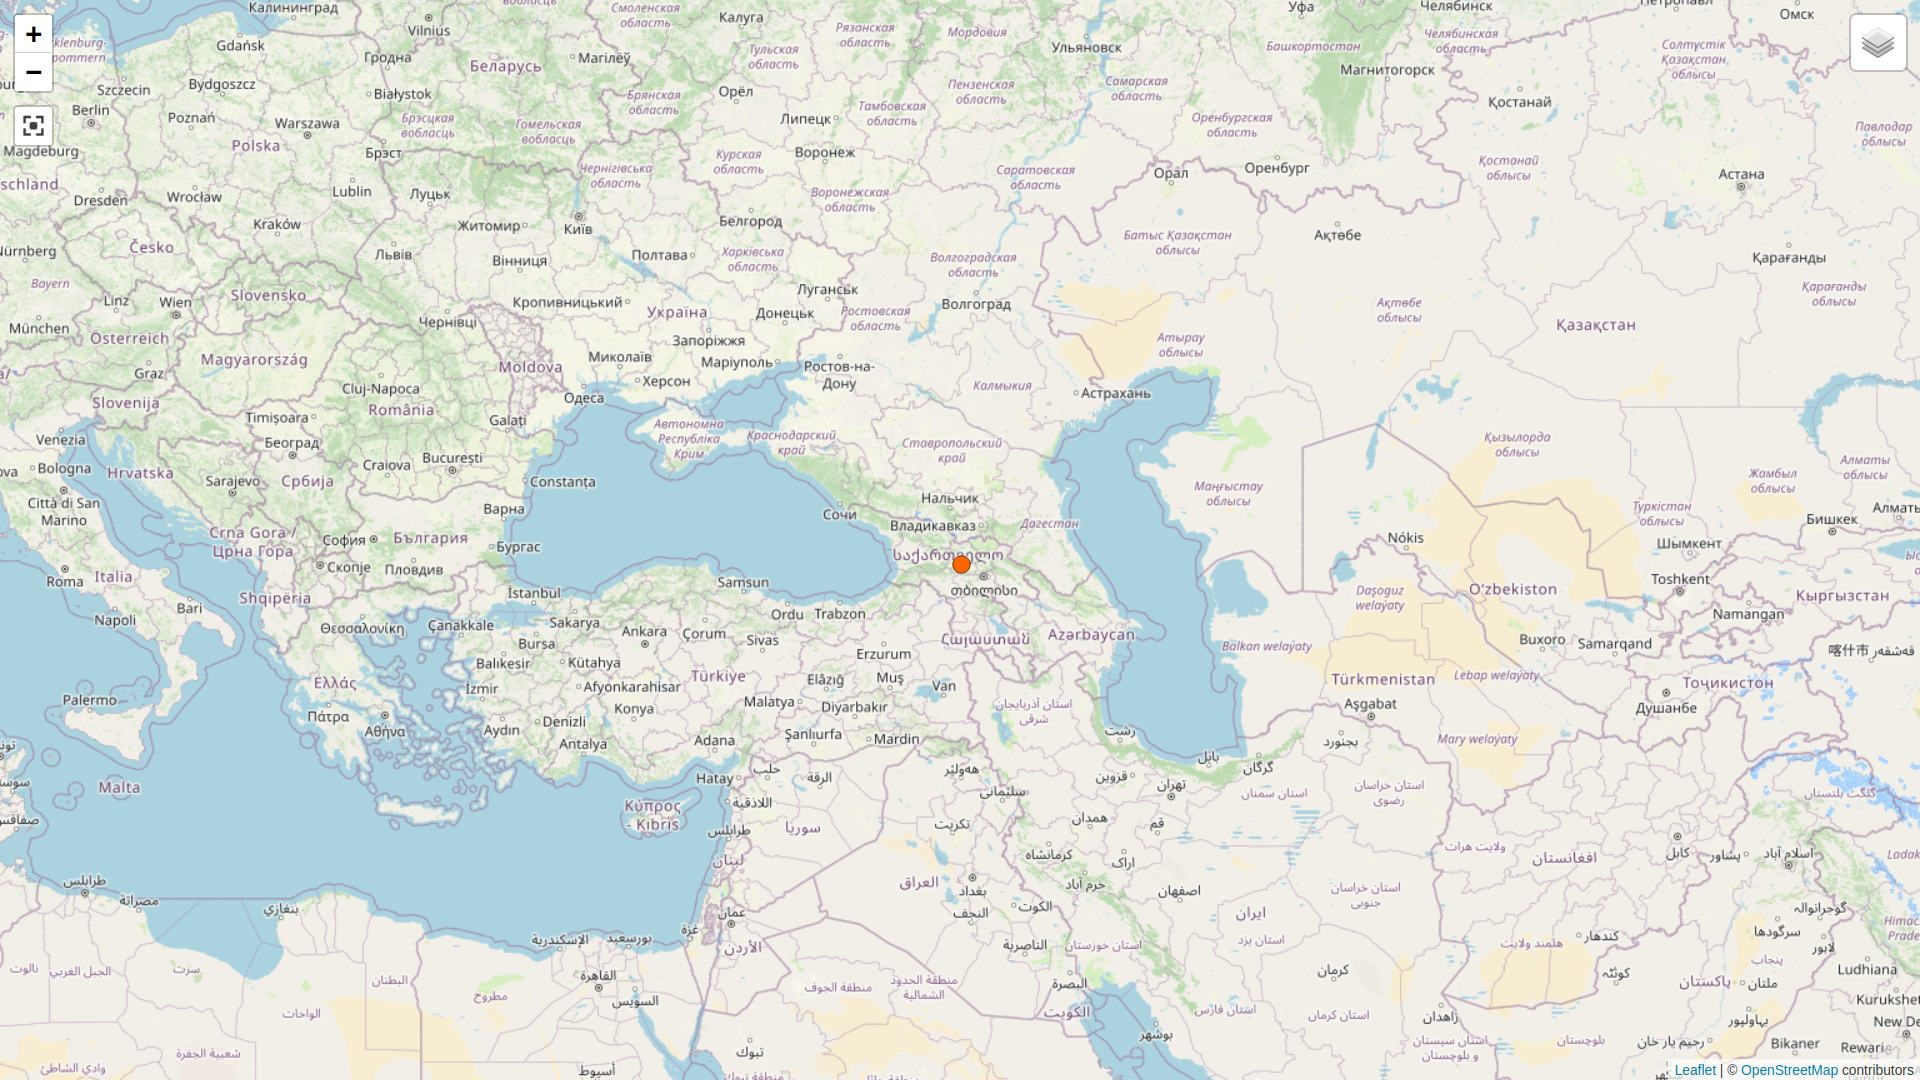
\includegraphics[scale=0.2]{./pics/urum_map_big.png}
\end{frame}

\begin{frame}[t]{Urum}
	\begin{itemize}
		\item<1->Kaukasisches Urum (nicht \textit{Crimean Urum})
		\item<2->Türkische Sprache gesprochen in Georgien (in den Hochlanden von of K’vemo K’art’li) u.a. am Fluss Tsalka
		\item<3-> Türkisch sprechende Pontogriechen, die Anatolien zu Beginn des 19. Jahrhundert verließen
		\item<4->Menschen mit griechischer Ethnizität in der Region Tsalka (die meisten sprechen Urum):
		\begin{itemize}
			\item<5->1979: 30.811
			\item<6->2002: 4.589
			\item<7->2005: 1.500
		\end{itemize}
		\item<8->Bilingual russisch (Urum enthält viele russische Lehnwörter bzw. Code Switching findet oft statt)
	\end{itemize}
\end{frame}

\begin{frame}[t]{Warum Urum?}
\begin{itemize}
	\item<1->NLP-Anwendung auf/für kleine, bedrohte Sprachen, was sonst selten bzw. (meiner Kenntnis nach) nicht existent ist.
	\item<2->Verwandt mit dem Türkischen; Vergleich mit Sprachmodellen des Türkischen
	\item<3->Kenntnisse für die Sprachdaten, aber auch die Sprache und ihre Struktur selbst erlangen.
	\item<4-> Mit NLP-Lösungen anderer, großer Sprachen vergleichen.
\end{itemize}
\end{frame}

\section{Was ist ein Hidden Markov Model (HMM)?}

\begin{frame}[t]{Was ist ein Hidden Markov Model (HMM)?}
\begin{itemize}
	\item<1->H = Hidden
	\begin{itemize}
		\item<6->Die betrachteten Zustände sind versteckt bzw. nicht direkt beobachtbar.
	\end{itemize}
	\item<1->M = Markov
	\begin{itemize}
		\item<3->Andrei Andrejewitsch Markow, russischer Mathematiker (1856-1922); Vorhersage von Zuständen basiert auf folgender Annahme:
		\item<4->\textbf{Markov Annahme}: $P(q_i = a|q_i...q_{i-1}) = P(q_i = a|q_{i-1})$\\\onslide<5->{
		Die Wahrscheinlichkeit eines Zustandes $q_i$ innerhalb einer Kette vorheriger Zustände $q_1...q_{i-1}$ wird einzig auf Basis der Wahrscheinlichkeit des vorherigen Zustandes $q_{i-1}$ berechnet.}
	\end{itemize}
	\item<1->M = Model
	\begin{itemize}
		\item<2->Stochastisches Modell zur Vorhersage von Zustandsabfolgen (sogenannten \textbf{Markovketten}). Bspw. Wetter, ob der Bus kommt.
	\end{itemize}
\end{itemize}
\end{frame}

\begin{frame}{Hidden Markov Model}
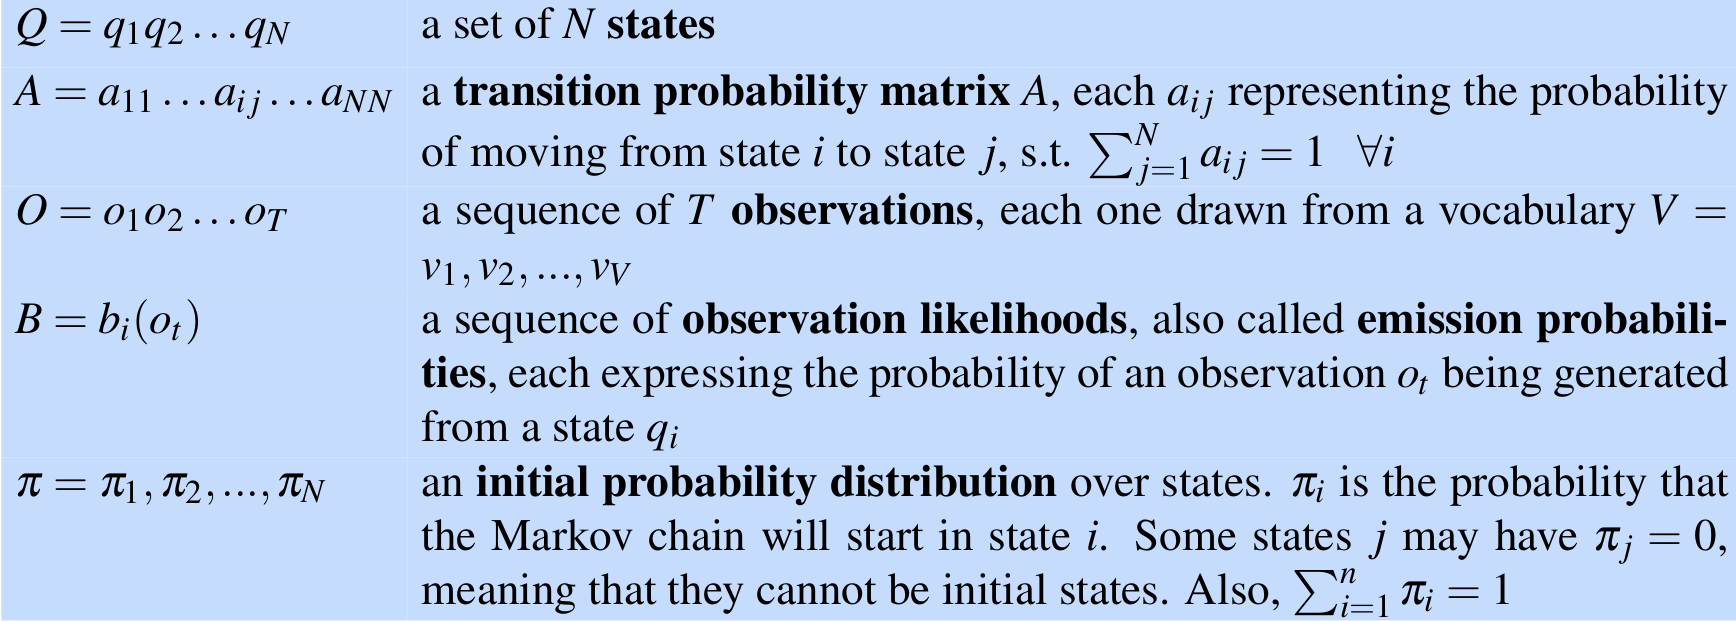
\includegraphics[scale=0.32]{"./pics/hmm_definition.png"}
\end{frame}

\section[t]{HMM als POS-Tagger}

\begin{frame}[t]{Beispiel eines HMM als POS-Tagger}
\begin{itemize}
	\item<1->Beobachtungen = folgende Sätze:
	\begin{itemize}
		\item<2-3>"Der Kundin gefällt das Haus ."
		\item<3>"Das ist schön ."
	\end{itemize}
\end{itemize}
\end{frame}

\begin{frame}[t]{Beispiel eines HMM als POS-Tagger}
	\begin{itemize}
		\item<1->Beobachtungen = folgende Wort-Wortart-Paarungen:
		\begin{itemize}
			\item<1->"Das/D Haus/N gefällt/V der/D Kundin/N ./PNCT"
			\item<1->"Das/Pro ist/V schön/A ./PNCT"
		\end{itemize}
		\item<2->Zustände = \{D,N,V,A,Pro,PNCT\}
		\item<3->Emissionswahrscheinlichkeiten: \onslide<4->{$P(W|T) = C(\langle W,T\rangle)/C(T)$}
		
		\onslide<5->{\begin{tabular}[htbp!]{lllllll}
				&D&N&V&A&Pro&PNCT\\
			Das&\textbf{1/2}&0&0&0&\textbf{1/1}&0\\
			Haus&0&\textbf{1/2}&0&0&0&0\\
			gefällt&0&0&\textbf{1/2}&0&0&0\\
			der&\textbf{1/2}&0&0&0&0&0\\
			Kundin&0&\textbf{1/2}&0&0&0&0\\
			ist&0&0&\textbf{1/2}&0&0&0\\
			schön&0&0&0&\textbf{1/1}&0&0\\
			.&0&0&0&0&0&\textbf{2/2}\\
		\end{tabular}}
	\end{itemize}
\end{frame}

\begin{frame}[t]{Beispiel eines HMM als POS-Tagger}
	\begin{itemize}
	\item<1->Transitionswahrscheinlichkeiten:\smallskip
	
	\onslide<2->{$P(T_2|T_1) = C(\langle T_1,T_2\rangle)/C(T_1)$}
	\smallskip
	
	\begin{itemize}
		\item<3->\onslide<4->{\textbf{<S>}}Das/D Haus/N gefällt/V der/D Kundin/N ./PNCT\onslide<4->{\textbf{<E>}}
		\item<3->\onslide<4->{\textbf{<S>}}Das/Pro ist/V schön/A ./PNCT\onslide<4->{\textbf{<E>}}
	\end{itemize}
		\smallskip
		\onslide<5->{\begin{tabular}[htbp!]{ccccccccc}
				&<S>&D&N&V&A&Pro&PNCT&<E>\\
				<S>&0&\textbf{1/2}&0&0&0&\textbf{1/2}&0&0\\
				D&0&0&\textbf{2/2}&0&0&0&0&0\\
				N&0&0&0&\textbf{1/2}&0&0&\textbf{1/2}&0\\
				V&0&\textbf{1/2}&0&0&\textbf{1/2}&0&0&0\\
				A&0&0&0&0&0&0&\textbf{1/1}&0\\
				Pro&0&0&0&\textbf{1/1}&0&0&0&0\\
				PNCT&0&0&0&0&0&0&0&\textbf{2/2}\\
				<E>&0&0&0&0&0&0&0&0\\
		\end{tabular}}
	\end{itemize}
\end{frame}

\begin{frame}[t]{Beispielberechnung}
	\begin{itemize}
		\item<1-><S> Das Haus ist schön . <E>.
		\item<2-><S>-D\onslide<4->{-N}\onslide<6->{-V-A-.-<E>}
		\begin{itemize}
			\item<2->1/2*1/2\onslide<4->{ *1*1/2}\onslide<6->{ *1/2*1/2 *1/2*1 *1*1 *1 = 0,015625}
		\end{itemize}
		\item<3-><S>-Pro\onslide<5->{-N}
		\begin{itemize}
			\item<3->1/2*1\onslide<5->{ *\textbf{0}*1/2 = 0}
		\end{itemize}
	\end{itemize}
\end{frame}

\section{Meine Implementierung eines HMM als POS-Tagger für Urum}

\begin{frame}[t]{1. Skript: Wort-POS-Tag-Paare von Urum erhalten}
	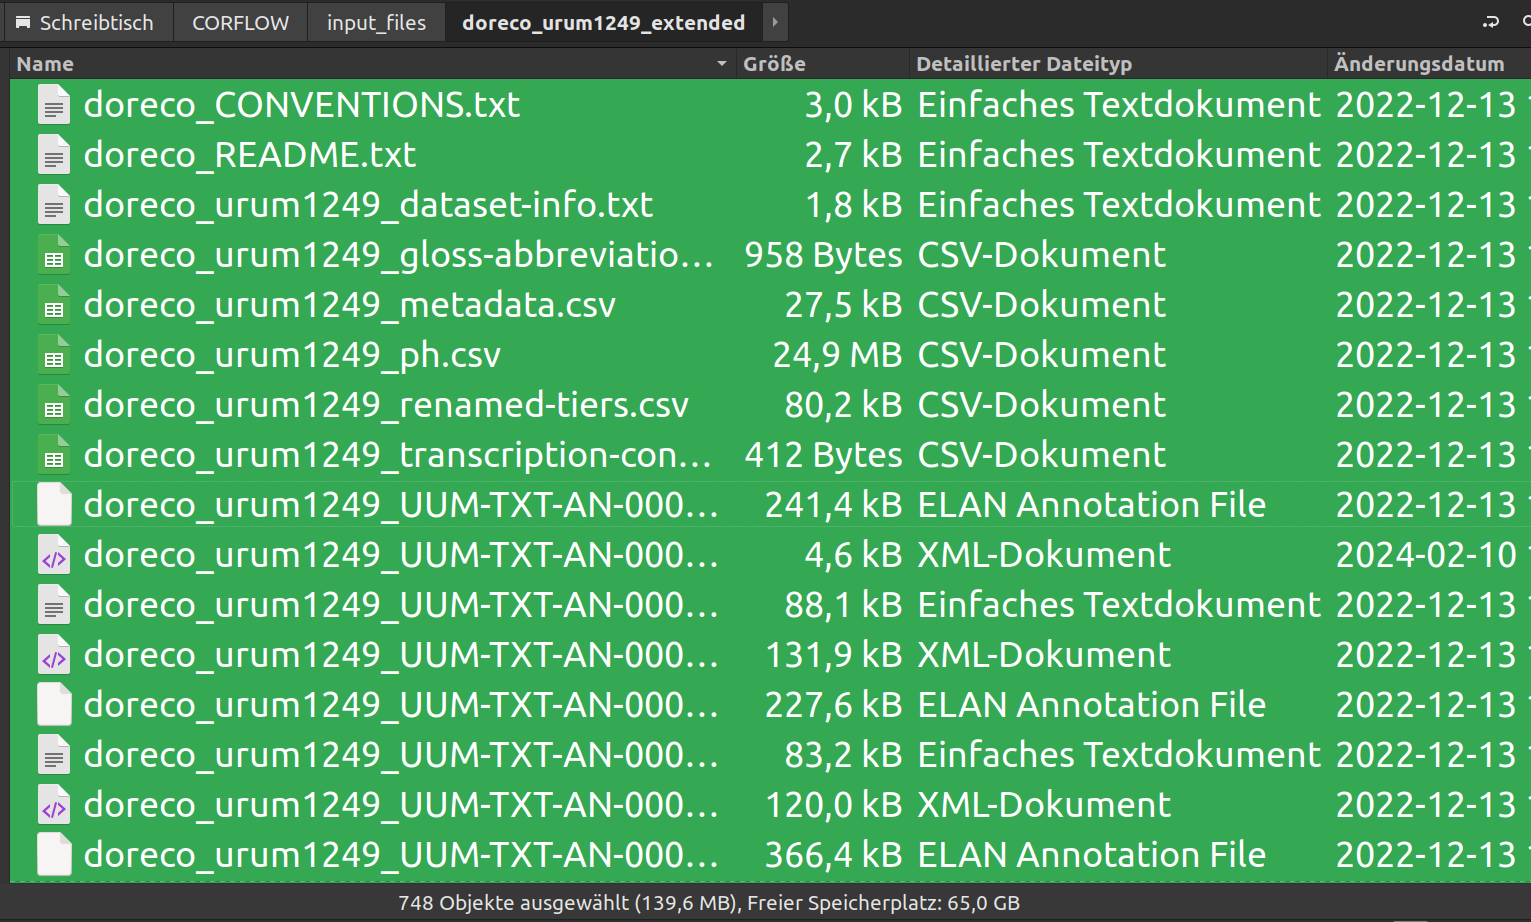
\includegraphics[scale=0.35]{"./pics/get_urum_script_pics/files.png"}
\end{frame}

\begin{frame}[t]{1. Skript: Wort-POS-Tag-Paare von Urum erhalten}
\includegraphics[scale=0.5]{"./pics/get_urum_script_pics/01.png"}
\includegraphics[scale=0.45]{"./pics/get_urum_script_pics/02.png"}
\end{frame}

\begin{frame}[t]{Ebenen und Segmente in ELAN}
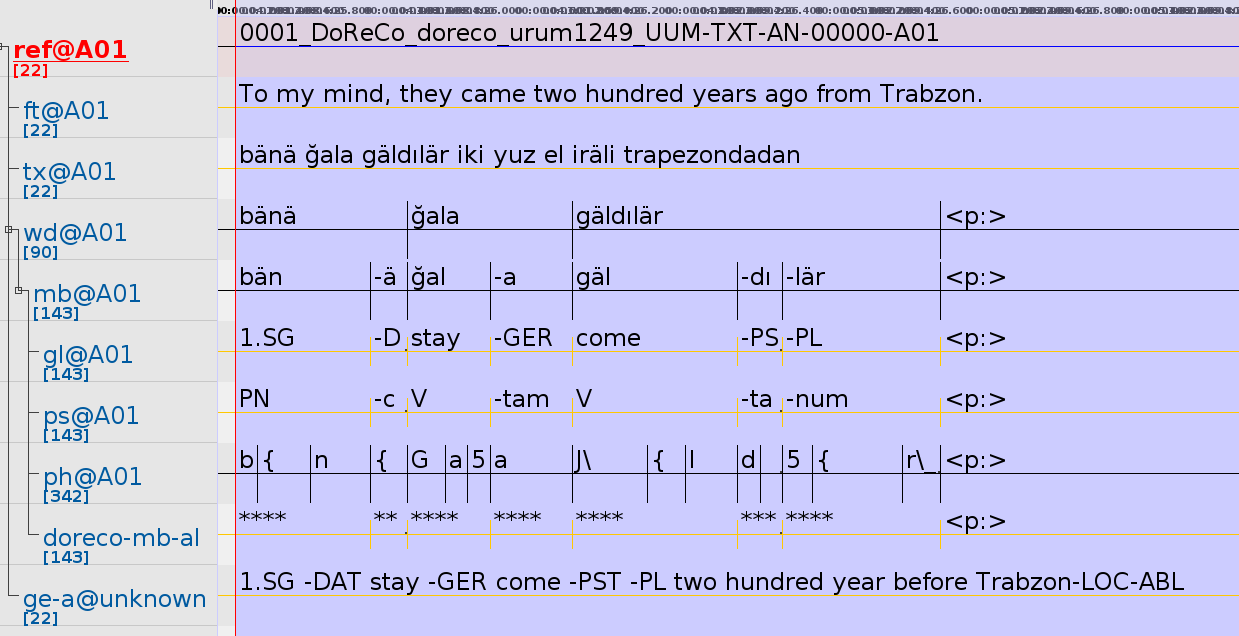
\includegraphics[scale=0.45]{./pics/urum_doreco_elan_example.png}
\end{frame}

\begin{frame}[t]{1. Skript: Wort-POS-Tag-Paare von Urum erhalten}
	\includegraphics[scale=0.45]{"./pics/get_urum_script_pics/03.png"}
\end{frame}

\begin{frame}[t]{1. Skript: Wort-POS-Tag-Paare von Urum erhalten}
	\includegraphics[scale=0.4]{"./pics/get_urum_script_pics/04.png"}
	
	\medskip
	\includegraphics[scale=0.45]{"./pics/get_urum_script_pics/05.png"}
	
	\includegraphics[scale=0.45]{"./pics/get_urum_script_pics/06.png"}
	\includegraphics[scale=0.45]{"./pics/get_urum_script_pics/07.png"}
\end{frame}

\begin{frame}[t]{2. Skript: HMM trainieren und testen}
	\includegraphics[scale=0.5]{"./pics/hmm_script_pics/01.png"}
	
	\medskip
	
	\includegraphics[scale=0.43]{"./pics/hmm_script_pics/02.png"}
	
	\medskip
	
	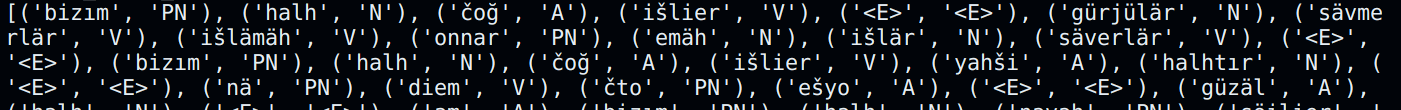
\includegraphics[scale=0.4]{"./pics/hmm_script_pics/14.png"}
\end{frame}

\begin{frame}[t]{2. Skript: HMM trainieren und testen}
	\includegraphics[scale=0.43]{"./pics/hmm_script_pics/03.png"}
	
	\medskip
	
	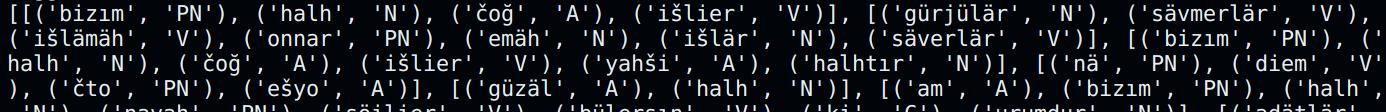
\includegraphics[scale=0.4]{"./pics/hmm_script_pics/15.png"}
\end{frame}


\begin{frame}[t]{2. Skript: HMM trainieren und testen}
	\includegraphics[scale=0.43]{"./pics/hmm_script_pics/04.png"}
	
	\medskip
	
	\includegraphics[scale=0.4]{"./pics/hmm_script_pics/05.png"}
\end{frame}

\begin{frame}[t]{2. Skript: HMM trainieren und testen}
	\includegraphics[scale=0.43]{"./pics/hmm_script_pics/06.png"}
\end{frame}

\begin{frame}[t]{2. Skript: HMM trainieren und testen}
	\includegraphics[scale=0.43]{"./pics/hmm_script_pics/07.png"}
\end{frame}

\begin{frame}[t]{2. Skript: HMM trainieren und testen}
	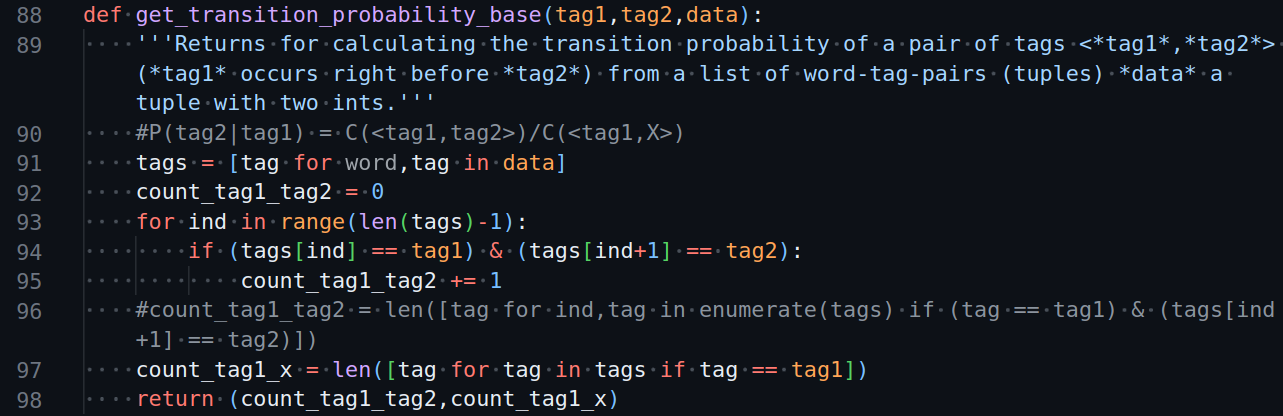
\includegraphics[scale=0.43]{"./pics/hmm_script_pics/08.png"}
\end{frame}

\begin{frame}[t]{2. Skript: HMM trainieren und testen}
	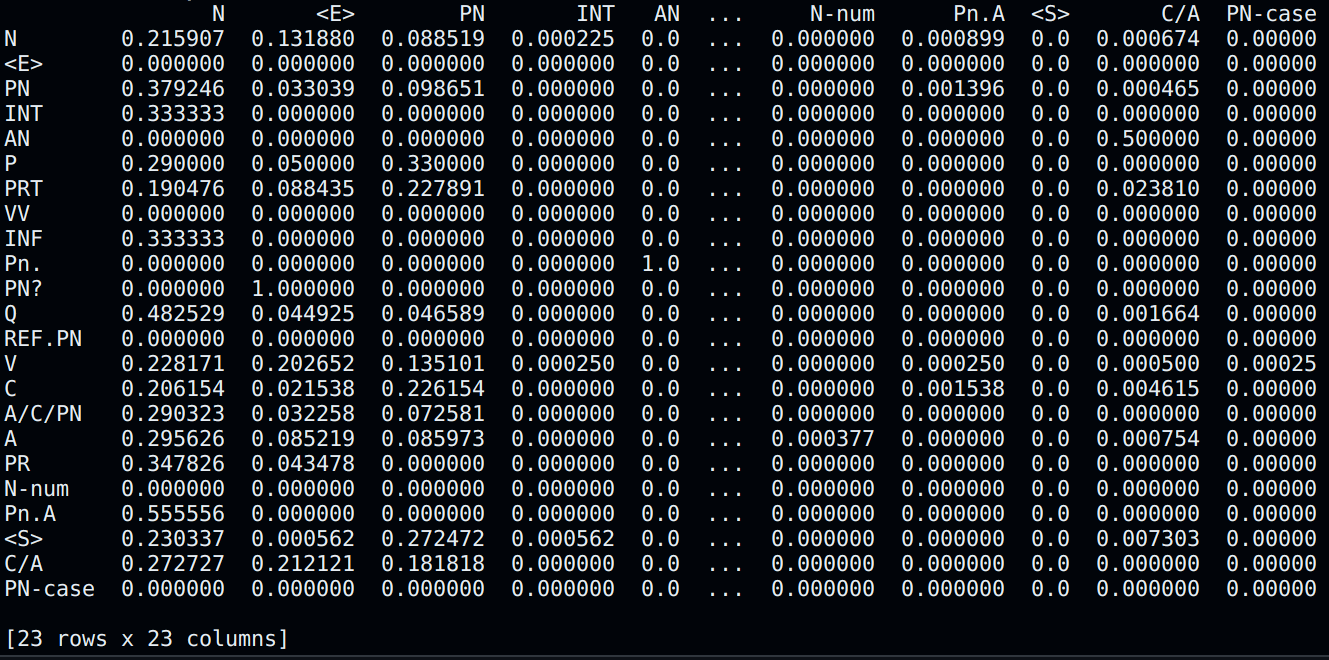
\includegraphics[scale=0.43]{"./pics/hmm_script_pics/16.png"}
\end{frame}

\begin{frame}[t]{2. Skript: HMM trainieren und testen}
	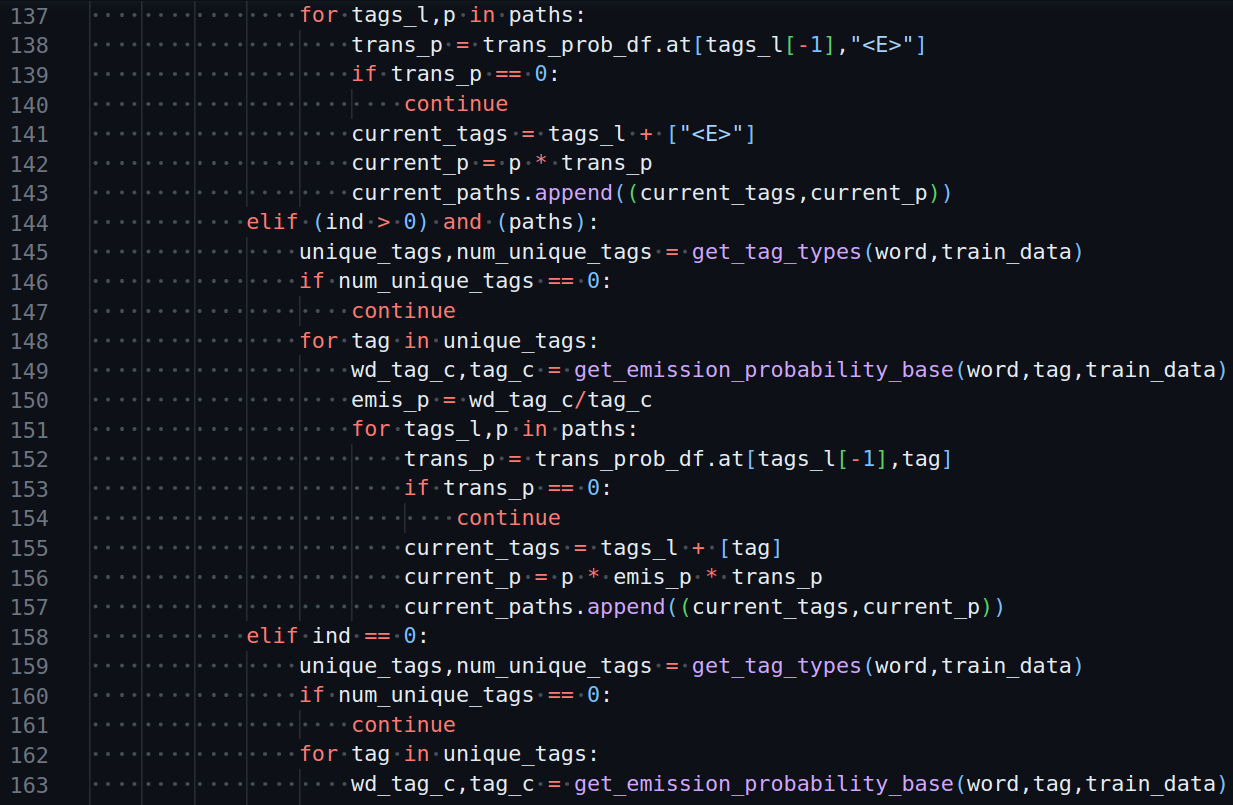
\includegraphics[scale=0.43]{"./pics/hmm_script_pics/11.png"}
\end{frame}

\begin{frame}[t]{2. Skript: HMM trainieren und testen}
	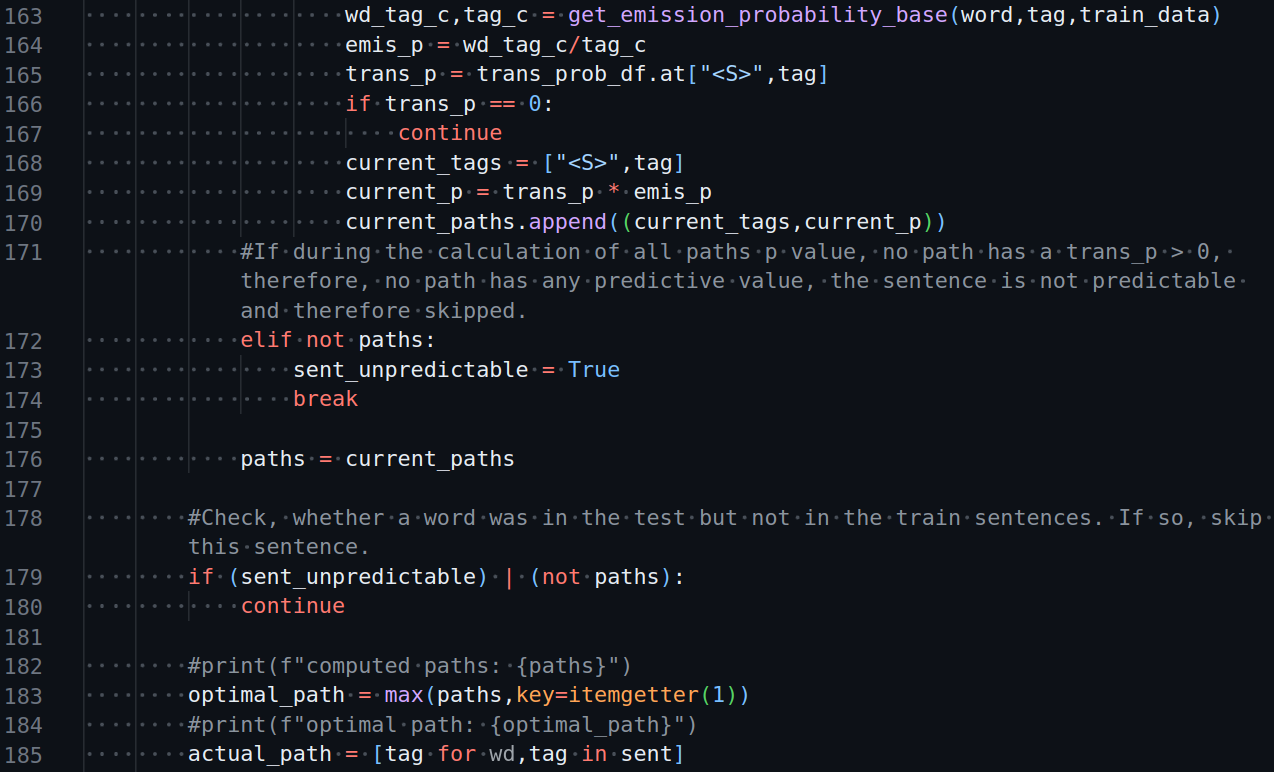
\includegraphics[scale=0.43]{"./pics/hmm_script_pics/12.png"}
\end{frame}

\begin{frame}[t]{2. Skript: HMM trainieren und testen}
	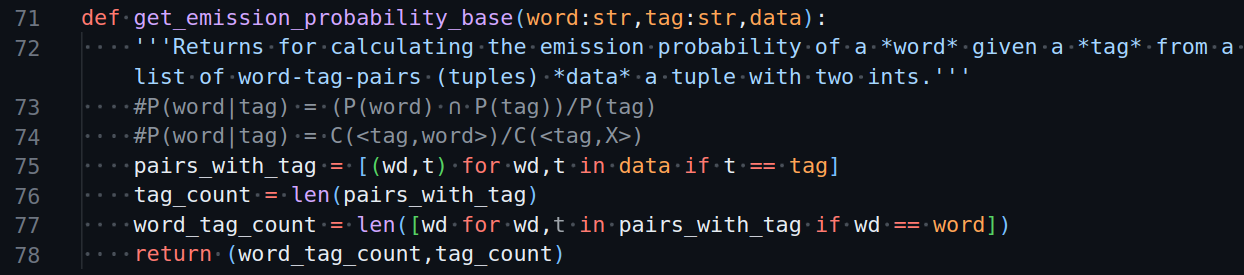
\includegraphics[scale=0.43]{"./pics/hmm_script_pics/10.png"}
	
	\medskip
	
	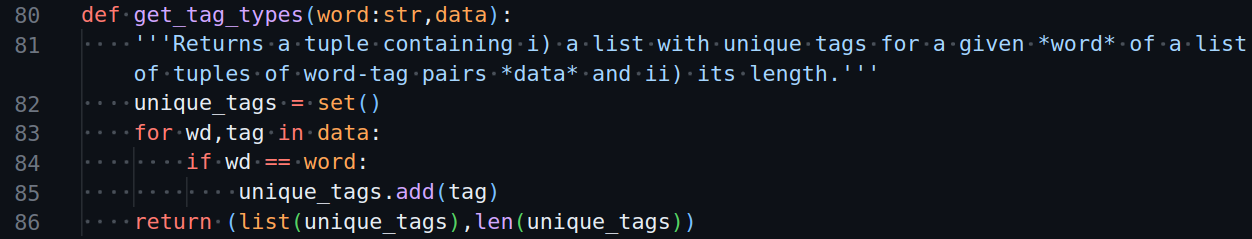
\includegraphics[scale=0.43]{"./pics/hmm_script_pics/09.png"}
\end{frame}

\begin{frame}[t]{2. Skript: HMM trainieren und testen}
	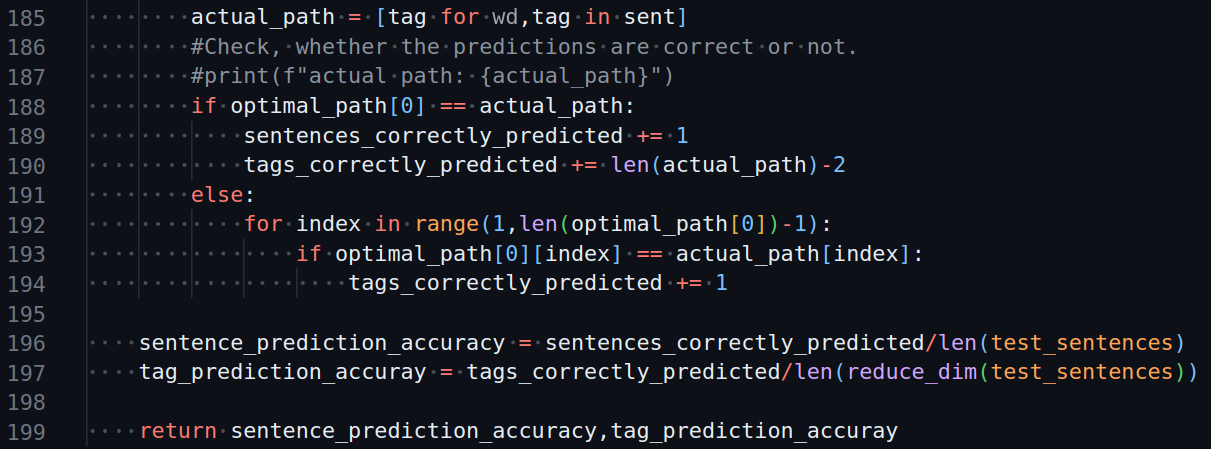
\includegraphics[scale=0.43]{"./pics/hmm_script_pics/13.png"}
	
	\medskip
	
	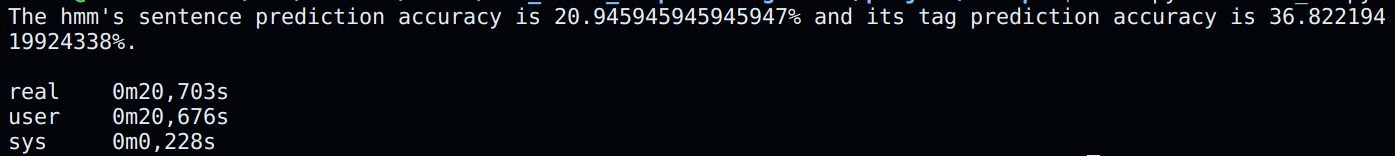
\includegraphics[scale=0.4]{"./pics/hmm_script_pics/17.png"}
\end{frame}

\begin{frame}[t]{Referenzen}
	\begin{itemize}
		\item Jurafsky, Daniel and Martin, James H. (2024): Speech and Language Processing. Draft of February 3, 2024.
		\item Great Learning Team (2022): Part of Speech (POS) tagging with Hidden Markov Model. URL: <https://www.mygreatlearning.com/blog/pos-tagging/> (zuletzt aufgerufen am 10.02.2024).
		\item Skopeteas, Stavros (2015): Caucasian Urums and Urum language.
		\item DoReCo Projekt Webseite. URL: <https://doreco.info/> (zuletzt aufgerufen am 10.02.2024).
		\item DoReCo Sprachdaten Webseite. URL: <https://doreco.huma-num.fr> (zuletzt aufgerufen am 10.02.2024).
	\end{itemize}
\end{frame}

\end{document}

